%---------- Quinto Capítulo: Desenvolvimento do Software ----------
\chapter{Desenvolvimento do Software}
\label{chap:desenv}

Utilizando a metodologia e o projeto do sistema apresentados nos capítulos \ref{metod} e \ref{specs}, respectivamente, inicou-se o desenvolvimento efetivo do sistema.
Primeiramente foi criado um projeto Maven principal denominado \texttt{onibuscerto}, o qual foi dividido em quatro subprojetos: 
\begin{itemize}
	\item \texttt{onibuscerto-api}: contém a classe que representa coordenadas geográficas e o objeto resposta contendo informações da rota ao Cliente.
	\item \texttt{onibuscerto-core}: consiste no módulo \emph{Core} definido no projeto do software (seção \ref{specs}). 
	Contém as representações das entidades originárias dos arquivos GTFS e faz interface do sistema com o banco de dados.
	\item \texttt{onibuscerto-importer}: consiste no módulo \emph{Importer} definido no projeto do software (seção \ref{specs}).
	Responsável pela importação dos dados contidos nos arquivos GTFS para o sistema através das funcionalidades do \emph{Core}.
	\item \texttt{onibuscerto-service}: consiste nos módulos \emph{Web Service} e Cliente definidos na seção \ref{specs}. 
	Pretende-se futuramente separar este subprojeto em dois outros distintos representando tais módulos.
\end{itemize}

Nas subseções a seguir serão descritos detalhes a respeito da implementação de cada subprojeto.

\section{Configuração do ambiente de desenvolvimento}

\section{onibuscerto-core}

O \emph{Core} consiste basicamente na interface do sistema com o banco de dados, contendo portanto as representações das entidades originárias dos arquivos GTFS.
Estas representações nada mais são do que \emph{wrappers}, ou seja, classes no sistema que são responsáveis pelo encapsulamento das entidades do banco de dados.
Cada uma destas classes é implementação de uma respectiva interface, e tem o intuito de referenciar um nó ou aresta do grafo armazenado.

O \emph{Core} foi organizado de tal forma que todas as suas classes de entidades possuam suas respectivas \emph{factories}.
Como já comentado, \emph{factory} consiste em uma interface com o objetivo de criação de famílias de objetos dependentes ou correlacionados.
Desta forma, toda criação de entidades é realizada através de uma \emph{factory}, centralizando este processo a somente uma classe por entidade.

Cada \emph{factory} de entidade pertencente ao arquivo GTFS é armazenada no banco de dados como um nó de referência, o qual possui uma relação para cada nó de sua respectiva entidade.
Esta organização das \emph{factories} no grafo pode ser observada na figura \ref{fig:grafoFactory}.

\begin{figure}[!htb]
	\centering
	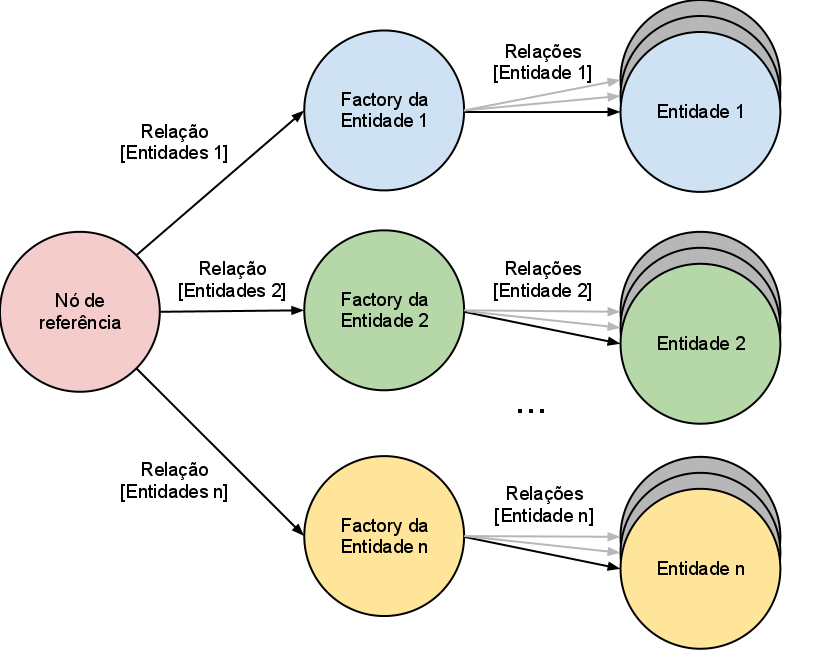
\includegraphics[width=0.7\textwidth]{./imgs/grafoFactory.png}
	\caption[Arquitetura do sistema]{Visão geral da organização das \emph{factories} do grafo.}
	\fonte{Autoria Própria}
	\label{fig:grafoFactory}
\end{figure}

A partir do nó de referência do grafo tem-se relações às \emph{factories} de todas as entidades (relação no formato [Entidades X]), sendo que estas tem relações a cada nó de seu tipo entidade (relação no formato [Entidade X]).
Com estas relações, a \emph{factory} pode ser utilizada para acessar todas as entidades do mesmo tipo, bastando percorrer o grafo.

O uso deste tipo de arquitetura torna o sistema flexível quanto ao SGBD, sendo que se necessária alguma modificação basta atualizar as \emph{factories} de acordo com o novo banco de dados. 
A seguir serão descritas todas as entidades pertencentes ao sistema, bem como a classe responsável pela interface com o banco de dados.

\subsection{Entidades}
As entidades que compõem o \emph{Core}, juntamente com suas \emph{factories}, são representadas através de interfaces e suas respectivas implementações por meio de classes no sistema.
As interfaces que representam as entidades e suas \emph{factories} pertencem ao pacote \texttt{com.onibuscerto.core.entities} e \texttt{com.onibuscerto.core.factories}, respectivamente.
Já as implementações das mesmas estão localizadas no pacote \texttt{com.onibuscerto.core}.

A seguir serão descritos detalhes de implementação das classes que encapsulam as entidades, as quais em conjunto formam o grafo armazenado no banco de dados do sistema.

\subsubsection{Location}
Entidade responsável principalmente por representar pontos através de coordenadas geográficas, bem como suas conexões com outros pontos.
Contém basicamente em quatro atributos: latitude, longitude, coleção de conexões chegando e saindo da \emph{Location}.
Estas propriedades são armazenadas no próprio nó do grafo através de pares chave/valor, sendo estas disponíveis para futuras consultas.

A \emph{factory} assignada a esta entidade denomina-se \emph{LocationFactory} e tem as funcionalidades de:
\begin{itemize}
	\item criar todas as entidades do tipo \emph{Location}, inclusive  suas extensões, como é o caso da entidade \emph{Stop} descrita na subseção a seguir.
	\item retornar todas as \emph{Stops} do sistema.
	\item retornar uma determinada \emph{Stop} com base em sua ID.
\end{itemize}

Esta entidade é utilizada principalmente para demarcar os pontos de origem e destino fornecidos pelo usuário que não consistem em uma parada para embarque e desembarque de passageiros.
Esta demarcação é importante para que estes pontos sejam adicionados ao grafo, desta forma contribuindo para um melhor refinamento na busca da rota com tempo de viagem mínimo.

\subsubsection{Stop}

\subsubsection{Route}

\subsubsection{Trip}

\subsubsection{StopTime}

\subsubsection{Connection}


\subsection{DatabaseController}


\section{onibuscerto-importer}

\section{onibuscerto-service}

O subprojeto \texttt{onibuscerto-service} é onde encontram-se os Servlets responsáveis por executar consultas na base de dados construída através do \emph{Importer}.
Os Servlets funcionam sob a forma de \emph{web services} e, sendo assim, todas as consultas são feitas pelos clientes através de requisições \sigla{HTTP}{Hypertext Transfer Protocol} do tipo GET ou POST.
As implementações dos Servlets residem no pacote \texttt{com.onibuscerto.service.servlets}.

Atualmente, apenas consultas que determinam a rota com o menor tempo de viagem entre duas coordenadas geográficas estão implementadas.
Estas consultas são de responsabilidade do Servlet implementado na classe \texttt{RouteServlet}.
No início do seu ciclo de vida, este é responsável por obter uma instância da classe \texttt{DatabaseController} do \emph{Core}, a qual será utilizada para acessar o banco de dados e resolver as consultas.
Em seguida, assim como um Servlet comum, este muda para um estado no qual está disponível para atender requisições dos clientes.
Por fim, ao ser destruído, o \texttt{RouteServlet} deve chamar o método \texttt{close} do \texttt{DatabaseController}, com o objetivo de fechar a conexão com o banco de dados.
O ciclo de vida completo de um Servlet é ilustrado na Figura \ref{fig:servletciclo}.

\begin{figure}[!htb]
	\centering
	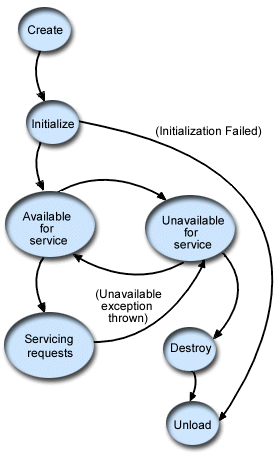
\includegraphics[width=0.4\textwidth]{./imgs/servletciclo.png}
	\caption[Ciclo de vida de um Servlet]{Ciclo de vida de um Servlet}
	\fonte{\citeonline{infocenter}}
	\label{fig:servletciclo}
\end{figure}

Enquanto o \texttt{RouteServlet} está ativo, ou seja, respondendo consultas, este recebe requisições HTTP do tipo POST com os seguintes parâmetros:
\begin{itemize}
	\item \texttt{start.latitude}: latitude do ponto de origem.
	\item \texttt{start.longitude}: longitude do ponto de origem.
	\item \texttt{end.lagitude}: lagitude do ponto de destino.
	\item \texttt{end.longitude}: longitude do ponto de destino.
	\item \texttt{departure}: horário de saída do ponto de origem, uma \emph{string} no formato \texttt{"HH:MM"}.
\end{itemize}

Ao receber estes parâmetros, o \texttt{RouteServlet} executa os seguintes passos:
\begin{enumerate}
	\item Converte as posições geográficas passadas como parâmetros para a consulta através de HTTP POST para objetos da classe \texttt{GlobalPosition}, do subprojeto \texttt{onibuscerto-api}.
	\item Cria nós no banco de dados para representar os nós de origem e destino, através da \texttt{LocationFactory}.
	\item Cria conexões do tipo \texttt{WalkingConnection} entre os recém-criados nós de origem e destino e todas as entidades do tipo \texttt{Stop} do grafo, de forma a representar os trechos que podem ser percorridos a pé pelo usuário.
	\item Executa a consulta no grafo através do método \texttt{getShortestPath} do \texttt{DatabaseController} e recebe o caminho encontrado sob a forma de um objeto do tipo \texttt{Collection<Connection>}.
	\item Converte o resultado da consulta para uma coleção de objetos da classe \texttt{QueryResponseConnection}, do subprojeto \texttt{onibuscerto-api}, ou seja, um objeto do tipo \texttt{Collection<QueryResposeConnection>}.
	\item Serializa o objeto \texttt{Collection<QueryResponseConnection>} para uma \emph{string} no formato \sigla{JSON}{JavaScript Object Notation}, o qual será finalmente enviado para o cliente do usuário.
\end{enumerate}

Tendo o funcionamento do \texttt{RouteServlet} em vista, a aplicação cliente é responsável apenas por enviar uma requisição HTTP POST para o serviço com os parâmetros no formato especificado e, por fim, interpretar os resultados retornados pelo servidor.
Uma pequena aplicação de exemplo que executa consultas no \emph{Service}, escrita em linguagem Python, é apresentada no Apêndice \ref{ape:exemplodeuso}.

\subsection{Cliente Web}

\section{Considerações}
